\section{Technischer Regelkreis}
\subsection{Definitionen \formelbuch{14}}

\begin{description}[leftmargin=2.5cm]
 \item[System] Eine Anordnung von Gebilden, die miteinander in Beziehung stehen
        	   und die sich gegenüber der Umgebung abgrenzen lasen.
 \item[Prozess] Die Gesammtheit der zusammenwirkenden Vorgänge in einem System,
        		durch die Materie, Energie, Informationen umgeformt, transportiert und
        		gespeichert wird.
 \item[SISO] Single Input - Single Output
 \item[MIMO] Multi Input - Multi Output
 \item[Steuerung] ohne Rückkopplung (open-loop)\newline
 				  - kann bei \textbf{stabiler} Strecke \textbf{nicht instabil} werden
 \item[Regelung] mit Rückkopplung (Gegenkopplung) (closed-loop) \newline
 				 - immer ein Vergleichsglied zwischen Führungsgrösse (Sollwert) und
 				 Regelgrösse (Istwert) \newline
 				 - kann auf veränderte Störgrössen reagieren \newline
 				 - kann bei \textbf{stabiler} Strecke \textbf{instabil} werden.
\end{description}

	\begin{tabular}{|p{2.7cm}|p{5.4cm}|l|}
    	\hline
    	{\bf Begriff deutsch}		&{\bf Begriff englisch}	&{\bf Ergänzende
    	Erklärung} \formelbuch{20}\\
		\hline
		Regelung /
		Regelkreis			& closed loop control / control loop & \\
		\hline
		Regelstrecke
    	Reglekreis			&plant controlled system	&Der aufgabengemäss zu beeinflussende
    	Teil des Systems\\
    	\hline
    	Regler				&controller			&Bestehent aus Vergleichsglied und Regelglied\\
    	\hline
    	Regeleinrichtung	&controlling means&\\
    	\hline
    	Reglesignalkreis	&control circuit&\\
    	\hline
    	Vergleichsglied		&comparing element	&Bildet den Fehler (Differenz)
    											e=r-y\\
    	\hline
    	Regelglied			&controller;
    						controlling element	&Berechnet aus dem Fehler die Stellgrösse u\\
    	\hline
    	Stelleinrichtung
    	Verstärker			&actuator;
					    	power amplifier;
    						servo amplifier		&Funktionseinheit, die den Energie- oder Massenstrom
    											lenkt\\
    	\hline
    	Messeinrichtung
    	Messumformer		&measuring unit;
    						transmitter&\\
    	\hline
    	Regelgrösse y		&controlled variable;
    						desiered value& auch c oder x (DIN)\\
    	\hline
    	Führungsgrösse r	&reference variable;
    						set value& w (DIN)\\
    	\hline
    	Störgrösse z Last	&disturbance variable;
    						load&\\
    	\hline
    	Stellgrösse u		&manipulatetd (correcting)
    						variable& y (DIN)\\
    	\hline
    	Regeldifferenz e
    	Fehler				&deviation;
    						error variable		&$e=r-y \quad \quad x_d=w-x$ (DIN) \\
    	\hline
    	Rückkopplung		&feedback			&Rückführung\\
    	\hline

	\end{tabular}\\
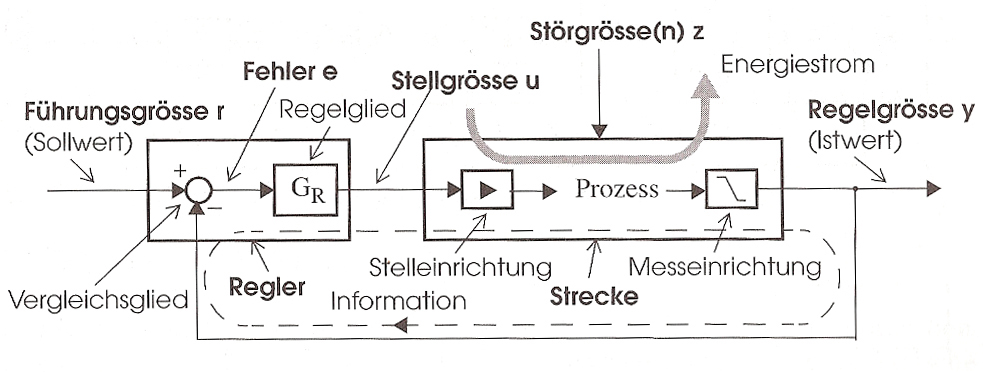
\includegraphics[height=4.5cm]{./bilder/Grundregelkreis_klein.jpg}


		
		\begin{sidewaystable}
		\subsection{Klassifizierung technischer Systeme}
		\begin{tabular}{|p{3cm}|p{2.5cm}|p{7cm}|p{11.5cm}|}
        	\hline
        	
        	einfach &
        	schwierig &
        	\textcolor{red}{\underline{für Regler}} &
        	Bedeutung des ersten Begriffs\\
        	\hline
        	
        	statisch &
        	\textcolor{red}{\underline{dynamisch}} &
        	&
        	Beschreiben nur den Gleichgewichtszustand (Vorgeschichte nicht
        	berücksichtigt)\\
        	\hline
        	
        	\textcolor{red}{\underline{linear}}	&
        	nichtlinear &
        	Ausnahmen: 2-, 3-Pt.Regler Simulation &
        	Assoziativ und Kommutativgesetz berücksichtigt \newline (x=X, 2x=2X;
        	y=Y, x+y=X+Y)\\
        	\hline
        	
        	\textcolor{red}{\underline{zeitinvariant}} &
        	zeitvariant &
        	&
        	unabhängig von zeitlicher Verschiebung \\
        	\hline
        	
        	\textcolor{red}{\underline{Zeitkontinuierlich}} &
        	zeitdiskret &
        	&
        	Signal hat zu jedem Zeitpunkt einen Wert\\
        	$\dot{y}=\frac{ku-y}{T}$ &
        	$y_{k+1}=a y_k + b u_k$	&
        	&
        	\\
        	\hline
        	
        	\textcolor{red}{\underline{wertkontinuierlich}}&
        	wertdiskret&
        	&
        	Signal kann alle Werte eines Intervalles annehmen\\
        	\hline
        	
        	\textcolor{red}{\underline{kausal}}	&
        	akausal	&
        	&
        	Gleiche Ursache führt zur gleichen Wirkung\\
        	\hline
        	
        	\textcolor{red}{\underline{konzentrierte}} &
        	verteilte &
        	zB.	Stromleitung: &
        	\\
        	\textcolor{red}{\underline{Parameter}} &
        	Parameter	&
        	ein R und ein C/ sehr viele RC-Glieder in Serie &
        	\\
        	\hline
        	
        	\textcolor{red}{\underline{deterministisch}}	&
        	stochastisch &
        	vorhersehbar/zufällig &
        	Das Zeitverhalten lässt sich aufgrund seiner Gleichungen
        	``reproduzieren"\\
        	\hline
        \end{tabular}
        \end{sidewaystable}